Onder de knop ``Opnames'' vindt U een overzicht van de pati\"enten
die in het ziekenhuis aanwezig zijn, in het verleden zijn opgenomen
of die ingepland zijn om in de toekomst opgenomen te worden.\\
\\
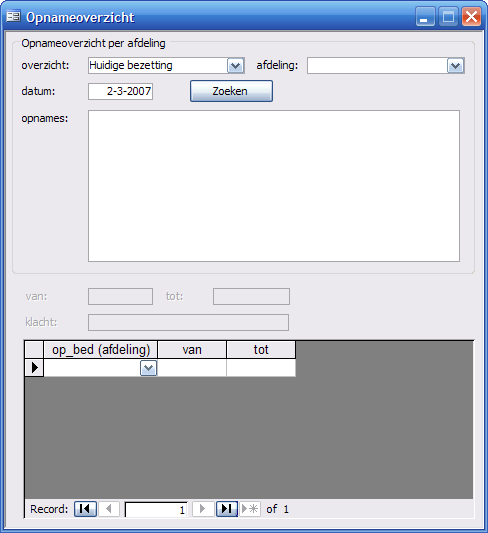
\includegraphics[scale=.5]{opnames1}

\section{Opnameoverzicht}\label{sec:opnameoverzicht} % (fold)

Er kunnen verschillende typen overzichten worden weergegeven. Kies
een type overzicht uit de lijst. Hieronder wordt meer uitgelegd over
de verschillende typen overzichten.

% section opnameoverzicht (end)

\section{Overzicht selecteren}\label{sec:overzicht selecteren} % (fold)

Om een overzicht van opnames te maken wordt er een datum ingevuld en
optioneel een afdeling. Als de naam van een afdeling wordt ingetypt
of geselecteerd uit een lijst, dan worden alleen de opnames van die
afdeling weergegeven. Als het tekstvak voor de afdeling wordt
leeggelaten, dan worden de opnames voor alle afdelingen weergegeven.
Om de pati\"enten weer te geven klikt U op de knop ``Zoeken''.

% section overzicht selecteren (end)

\section{Overzichtstypen}\label{sec:overzichtstypen} % (fold)

Er zijn vijf typen overzicht:
\begin{itemize}
  \item Huidige bezetting
  \item Huidige opnames
  \item Huidige ontslagen
  \item Afgehandelde opnames
  \item Toekomstige opnames
\end{itemize}

\subsection{Huidige bezetting}\label{sec:huidige bezetting} % (fold)
Alle pati\"enten die op de opgegeven datum in het ziekenhuis of op de geselecteerde afdeling aanwezig zijn worden weergegeven.
\subsection{Huidige opnames}\label{sec:huidige opnames} % (fold)
Alle pati\"enten die op de opgegeven datum in het ziekenhuis of op de geselecteerde afdeling opgenomen zullen worden.
\subsection{Huidige ontslagen}\label{sec:huidige ontslagen} % (fold)
Alle pati\"enten die op de opgegeven datum uit het ziekenhuis of van de geselecteerde afdeling ontslagen zullen worden.
\subsection{Afgehandelde opnames}\label{sec:afgehandelde opnames} % (fold)
Alle pati\"enten die voor de opgegeven datum in het ziekenhuis of op de geselecteerde afdeling een opname hebben gehad en zijn ontslagen.
\subsection{Huidige bezetting}\label{sec:huidige bezetting} % (fold)
Alle pati\"enten die op de opgegeven datum nog niet in het ziekenhuis of op de geselecteerde afdeling opgenomen zijn en waarvoor in de toekomst een opname gepland staat.

% section overzichtstypen (end)

\section{Detailvenster}\label{sec:detailvenster} % (fold)

Details over de opnames bij de case waarvoor de geselecteerde
pati\"ent is opgenomen kunnen in het detailvenster worden bekeken en
aangepast.

% section detailvenster (end)
